\documentclass[border=1.5pt]{standalone}
\usepackage{amsmath,amssymb}
\usepackage{tikz}
\usetikzlibrary{arrows.meta,calc,positioning,shapes,shapes.misc,shapes.geometric,backgrounds,fit,decorations.pathreplacing,quantikz2}
% Shared colors and styles for the XYZ^2 figures.
% Pauli types: bright tones for fills and bands, deep (800) shades of the same hues for labels.
% The label shades keep the hue of each Pauli, are well separated from each other (CIEDE2000 > 20)
% and have a contrast ratio of at least 2.9 on the coral cells and 4.5 on the sunflower cells.
\definecolor{PauliX}{HTML}{F97316}
\definecolor{PauliY}{HTML}{EC4899}
\definecolor{PauliZ}{HTML}{9333EA}
\definecolor{PauliXText}{HTML}{AC340B}
\definecolor{PauliYText}{HTML}{9D174D}
\definecolor{PauliZText}{HTML}{5B21B6}
% Generator classes: S0 (class B, even links, coral) and gauge (class A, odd links, sunflower)
\definecolor{Szero}{HTML}{F0435E}
\definecolor{SzeroText}{HTML}{BE123C}
\definecolor{Gauge}{HTML}{F59E0B}
\definecolor{GaugeText}{HTML}{B45309}
\colorlet{GaugeGray}{Gauge}
\definecolor{ClassB}{HTML}{FF8A99}
\definecolor{ClassA}{HTML}{FFD23F}
% Logical operators (X-bar violet, Z-bar crimson), errors, ink
\definecolor{LogicalZ}{HTML}{E11D48}
\definecolor{LogicalGold}{HTML}{7C3AED}
\definecolor{ErrRed}{HTML}{1C1917}
\definecolor{InkDark}{HTML}{292524}
\definecolor{InkSoft}{HTML}{57534E}
% Labels drawn on top of colored cells
\colorlet{CellText}{InkDark}
% Noise channels
\definecolor{ErrFlip}{HTML}{EF4444}
\definecolor{Idle}{HTML}{EC4899}
\definecolor{TwoQ}{HTML}{7C3AED}
% Protocol steps
\definecolor{StepPrep}{HTML}{F97316}
\definecolor{StepMeas}{HTML}{D946EF}
\definecolor{StepDec}{HTML}{7C3AED}
\definecolor{StepRec}{HTML}{DB2777}
\tikzset{
  qb/.style={circle, draw=InkDark, line width=0.6pt, fill=white,
             minimum size=4.2mm, inner sep=0pt, font=\scriptsize},
  qbsmall/.style={circle, draw=InkDark, line width=0.5pt, fill=white,
             minimum size=2.6mm, inner sep=0pt},
  hexedge/.style={line width=0.65pt, draw=InkSoft},
  linkedge/.style={line width=1.6pt, draw=InkDark},
  bndedge/.style={line width=0.65pt, draw=InkSoft, densely dashed},
  plabel/.style={font=\scriptsize\bfseries, inner sep=1pt},
  panel/.style={font=\small\bfseries, anchor=north west},
}

\providecommand{\ket}[1]{\left|#1\right\rangle}

\begin{document}
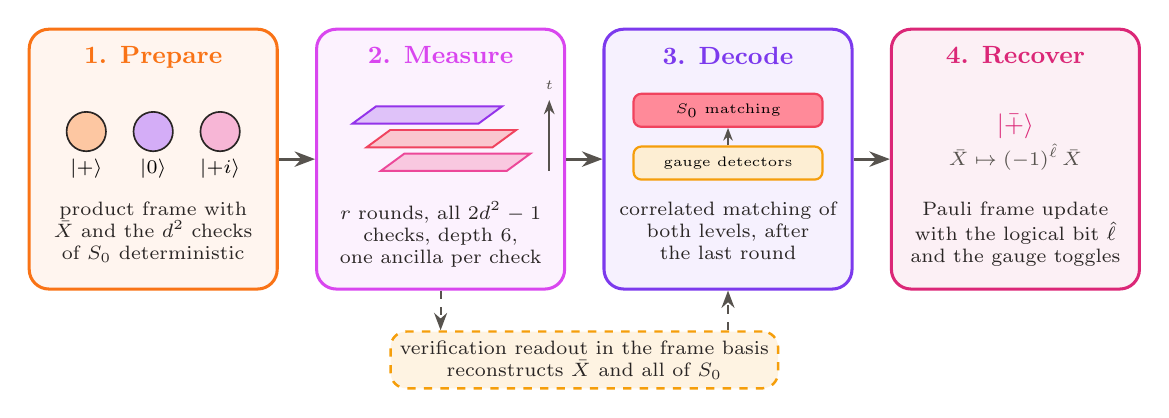
\begin{tikzpicture}[
  stage/.style={draw=#1, line width=1.1pt, rounded corners=2.5mm, fill=#1!7,
                minimum width=3.15cm, minimum height=3.3cm},
  stitle/.style={font=\small\bfseries, text=#1},
  stext/.style={font=\scriptsize, text=InkDark, align=center, text width=2.9cm},
  flow/.style={-{Stealth[length=2.6mm]}, line width=1.1pt, draw=InkSoft},
]
% ---------- stage boxes
\node[stage=StepPrep] (P) at (0,0) {};
\node[stage=StepMeas] (M) at (3.65,0) {};
\node[stage=StepDec] (D) at (7.30,0) {};
\node[stage=StepRec] (R) at (10.95,0) {};
\node[stitle=StepPrep, anchor=north] at ($(P.north)+(0,-0.12)$) {1. Prepare};
\node[stitle=StepMeas, anchor=north] at ($(M.north)+(0,-0.12)$) {2. Measure};
\node[stitle=StepDec, anchor=north] at ($(D.north)+(0,-0.12)$) {3. Decode};
\node[stitle=StepRec, anchor=north] at ($(R.north)+(0,-0.12)$) {4. Recover};
\draw[flow] (P.east) -- (M.west);
\draw[flow] (M.east) -- (D.west);
\draw[flow] (D.east) -- (R.west);
% ---------- stage 1: frame product state (three single-qubit states)
\begin{scope}[shift={(P.center)}]
  \node[qb, fill=PauliX!40, minimum size=5mm] at (-0.85,0.35) {};
  \node[qb, fill=PauliZ!40, minimum size=5mm] at (0,0.35) {};
  \node[qb, fill=PauliY!40, minimum size=5mm] at (0.85,0.35) {};
  \node[font=\scriptsize] at (-0.85,-0.12) {$|{+}\rangle$};
  \node[font=\scriptsize] at (0,-0.12) {$|0\rangle$};
  \node[font=\scriptsize] at (0.85,-0.12) {$|{+i}\rangle$};
  \node[stext, anchor=north] at (0,-0.42) {product frame with\\ $\bar X$ and the $d^2$ checks\\ of $S_0$ deterministic};
\end{scope}
% ---------- stage 2: rounds stacked in time
\begin{scope}[shift={(M.center)}]
  \foreach \k/\o/\c in {0/0.45/PauliZ,1/0.15/Szero,2/-0.15/PauliY}{
    \draw[fill=\c!30, draw=\c, line width=0.7pt]
      (-1.12+0.18*\k,\o) -- (0.48+0.18*\k,\o) -- (0.78+0.18*\k,\o+0.22) -- (-0.82+0.18*\k,\o+0.22) -- cycle;
  }
  \draw[-{Stealth[length=1.8mm]}, InkSoft, line width=0.8pt] (1.38,-0.15) -- (1.38,0.75) node[above, font=\tiny] {$t$};
  \node[stext, anchor=north] at (0,-0.42) {$r$ rounds, all $2d^2-1$\\ checks, depth 6,\\ one ancilla per check};
\end{scope}
% ---------- stage 3: two levels
\begin{scope}[shift={(D.center)}]
  \node[draw=Gauge, fill=Gauge!18, line width=0.8pt, rounded corners=1mm, font=\tiny, minimum width=2.4cm, minimum height=0.42cm] (lo) at (0,-0.05) {gauge detectors};
  \node[draw=Szero, fill=ClassB, line width=0.8pt, rounded corners=1mm, font=\tiny, minimum width=2.4cm, minimum height=0.42cm] (up) at (0,0.62) {$S_0$ matching};
  \draw[-{Stealth[length=1.6mm]}, line width=0.8pt, draw=InkSoft] (lo.north) -- (up.south);
  \node[stext, anchor=north] at (0,-0.42) {correlated matching of\\ both levels, after\\ the last round};
\end{scope}
% ---------- stage 4: recover
\begin{scope}[shift={(R.center)}]
  \node[font=\small, text=StepRec] at (0,0.42) {$|\bar{+}\rangle$};
  \node[font=\scriptsize, text=InkSoft] at (0,0.02) {$\bar X \mapsto (-1)^{\hat\ell}\,\bar X$};
  \node[stext, anchor=north] at (0,-0.42) {Pauli frame update\\ with the logical bit $\hat\ell$\\ and the gauge toggles};
\end{scope}
% ---------- verification branch
\node[draw=Gauge, dashed, line width=0.9pt, rounded corners=2mm, font=\scriptsize, align=center, text=InkDark, fill=Gauge!12,
      minimum width=4.9cm] (V) at (5.475,-2.55) {verification readout in the frame basis\\ reconstructs $\bar X$ and all of $S_0$};
\draw[-{Stealth[length=2.2mm]}, line width=0.8pt, draw=InkSoft, dashed] (M.south) -- (M.south |- V.north);
\draw[-{Stealth[length=2.2mm]}, line width=0.8pt, draw=InkSoft, dashed] (D.south |- V.north) -- (D.south);
\end{tikzpicture}

\end{document}
